\chapter{MEV and PBS Architecture}
\section{Introduction}
MEV stands for maximum extractable value, which is the amount of value that can be captured by a miner or validator by manipulating the transactions in a block. MEV can be positive or negative, depending on whether the manipulation increases or decreases the total value of the block. MEV can also affect the security and fairness of the blockchain, as it creates incentives for miners or validators to behave in ways that may harm other users or the network.
Some examples of MEV are:
\begin{itemize}
	\item \textbf{DEX arbitrage:} This is when a miner or validator exploits the price differences between two decentralized exchanges (DEXs) by buying low on one and selling high on another. This can generate profit for the miner or validator, but also affect the prices and liquidity of the DEXs.
	\item \textbf{Liquidations:} This is when a miner or validator triggers the liquidation of an undercollateralized loan or position on a lending or trading platform. This can allow the miner or validator to claim a portion of the collateral or assets, but also cause losses for the borrower or trader.
	\item \textbf{Sandwich trading:} This is when a miner or validator inserts their own transaction between two other transactions that are related to each other. For example, if a user wants to buy a large amount of tokens on a DEX, a miner or validator can insert their own buy order before the user’s order and their own sell order after the user’s order. This can allow the miner or validator to buy low and sell high, but also increase the slippage and cost for the user.
	\item \textbf{NFT MEV:} This is when a miner or validator exploits the demand and scarcity of non-fungible tokens (NFTs) by influencing their creation, distribution, or sale. For example, a miner or validator can front-run an NFT minting transaction by creating their own NFT with the same attributes before the original transaction is confirmed. This can allow the miner or validator to claim a rare or valuable NFT, but also it reduces the uniqueness and value of the original NFT.
\end{itemize}
MEV can cause bad user experience on the blockchain, such as network congestion, high transaction fees, unfair ordering, and security risks. MEV can also affect the fairness and efficiency of decentralized applications, such as decentralized exchanges, lending platforms, and NFT markets.\\
Aequitas is a new class of consensus protocols that aim to achieve order-fairness in addition to consistency and liveness. Order-fairness is a property that ensures that the ordering of transactions in a block reflects the order in which they were submitted by the users, and not by the adversary or the leader. Aequitas protocols can be realized in a black-box way using existing broadcast and agreement primitives, or any consensus protocol, and work in both synchronous and asynchronous network models. \href{https://eprint.iacr.org/2020/269.pdf}{Aequitas protocols} are the first to achieve order-fairness for Byzantine consensus.
\section{Flashbots}
Flashbots is a project that aims to improve the transparency, fairness, and efficiency of the blockchain by providing a platform for users to communicate with validators directly and privately. Flashbots Protect is a service that allows users to send their transactions to Flashbots instead of the public mempool, where they are vulnerable to frontrunning and other forms of MEV extraction.\\
Figure \ref{fig:L22_f1} shows how the Flashbots Protect service works:
\begin{itemize}
	\item The user submits their transaction to Flashbots through a web interface or an API. The transaction is encrypted and signed by the user’s private key.
	\item The transaction is relayed to the Flashbots Network, which is a network of relay nodes that connect users and validators. The relay nodes verify the validity and profitability of the transaction and forward it to the validators who are running Flashbots software.
	\item The validators receive bundles of transactions from the relay nodes and select the most profitable ones to include in their blocks. The validators also pay a portion of their block reward to the relay nodes and the users as a fee for using Flashbots.
	\item The validators propose their blocks to the network as usual, but without revealing the contents of the transactions until they are confirmed. This prevents frontrunning bots from copying or manipulating the transactions before they are executed.
	\item The user’s transaction is executed on the blockchain without being exposed to MEV attacks. The user can also monitor the status of their transaction on the Flashbots dashboard.
\end{itemize}
\begin{center}
	\begin{figure}
		\centering
		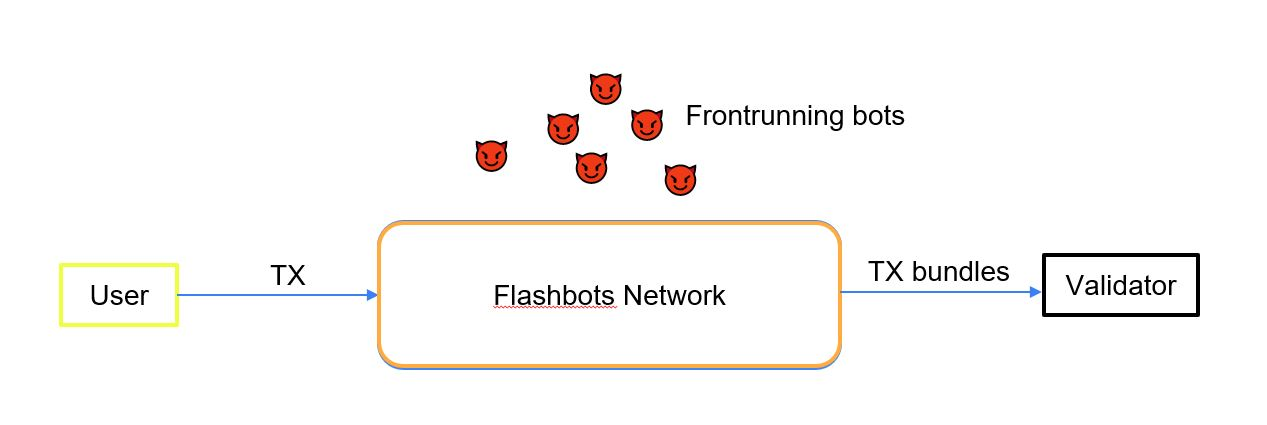
\includegraphics[width=0.8\linewidth]{Fig/22/F1}
		\caption{The diagram shows how the Flashbots Protect service works}
		\label{fig:L22_f1}
	\end{figure}
\end{center}
\section{MEV impacts on the consensus layer}
MEV can also affect the security and fairness of the blockchain, as it creates incentives for miners or validators to behave in ways that may harm other users or the network.\\
Some of the impacts of MEV on the consensus layer are:
\begin{enumerate}
	\item \textbf{Transaction censorship:} This is when a miner or validator deliberately excludes or delays certain transactions from being included in a block, based on their own preferences or incentives. For example, a miner or validator may censor transactions that compete with their own MEV opportunities, or transactions that are unfavorable to their political or economic interests. Transaction censorship can lead to validator centralization, as users may prefer to delegate their stake to validators who are more likely to include their transactions, creating a positive feedback loop for the dominant validators.
	\item \textbf{Staking inequality:} This is when a miner or validator has an unfair advantage over other miners or validators in terms of capturing MEV opportunities, due to their resources, connections, or strategies. For example, a large MEV pool may have more resources to invest in necessary optimizations to capture staking opportunities, such as faster hardware, better algorithms, or exclusive access to private transaction sources. Staking inequality can discourage solo stakers from participating in the network, as they may be unable to profit from MEV opportunities, reducing the decentralization and diversity of the network.
	\item \textbf{Re-org attacks:} This is when a miner or validator attempts to rewrite the history of the blockchain by creating a longer chain that replaces the existing chain, usually by withholding their blocks until they have enough proof-of-work or proof-of-stake to overtake the current chain. For example, if the MEV re-org in a block significantly exceeds the standard block reward, validators may be incentivized to forego blocks and capture the MEV for themselves, causing blockchain re-organization and consensus instability. Re-org attacks can undermine the trust and reliability of the blockchain, as users may lose confidence in the finality and validity of their transactions, see Figure \ref{fig:L22_f2}.
\end{enumerate}
\begin{center}
	\begin{figure}
		\centering
		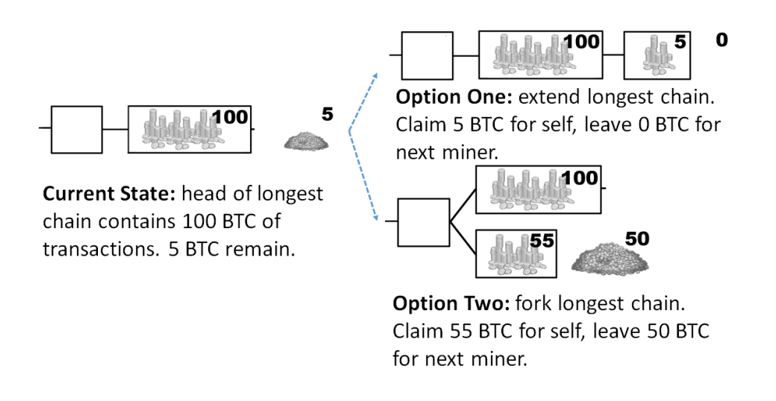
\includegraphics[width=0.8\linewidth]{Fig/22/F2}
		\caption{One possible state of blockchain and two possible actions a miner could take.}
		\label{fig:L22_f2}
	\end{figure}
\end{center}
\section{Proposer builder separation (PBS)}
Proposer-builder separation (PBS) is a way of separating the roles and responsibilities of block producers and block proposers on the blockchain. Block producers are the nodes that validate and finalize the blocks, while block proposers are the nodes that collect and order the transactions in the blocks. PBS aims to firewall MEV concerns away from the core protocol, by allowing block proposers to compete for MEV opportunities without affecting the block producers’ incentives or behavior.\\
The main benefits of PBS are:
\begin{itemize}
	\item It reduces the risk of re-org attacks, as block producers have no incentive to fork the chain or withhold their blocks, since they do not benefit from MEV.
	\item It increases the decentralization and diversity of the network, as block proposers can be anyone who can submit valid transactions, regardless of their stake or resources.
	\item It improves the efficiency and scalability of the network, as block proposers can use different strategies and optimizations to order transactions, without compromising the consistency or liveness of the network.
\end{itemize}
\subsection{Implementation}
One possible way to implement PBS, which is to create a market for blockspace, where proposers can sell their blocks to builders who want to buy them. This way, proposers can compete for MEV opportunities without affecting the block producers’ incentives or behavior. The slide also shows a diagram of six blocks connected by lines, representing a possible state of the blockchain. The last block on the right is red and has a question mark on it, indicating that it is unknown or uncertain. This may imply that the slide is asking how to determine the price and allocation of blockspace in such a market.\\
One possible answer to this question is to use an auction mechanism, where proposers can bid for the right to propose the next block, and builders can bid for the right to build on top of the proposed block. The auction mechanism can be designed to achieve certain objectives, such as efficiency, fairness, or revenue maximization. For example, one could use a second-price sealed-bid auction, where proposers and builders submit their bids privately, and the winner pays the second-highest bid. This type of auction can encourage truthful bidding and allocate blockspace to the highest-valued users.
\begin{center}
	\begin{figure}
		\centering
		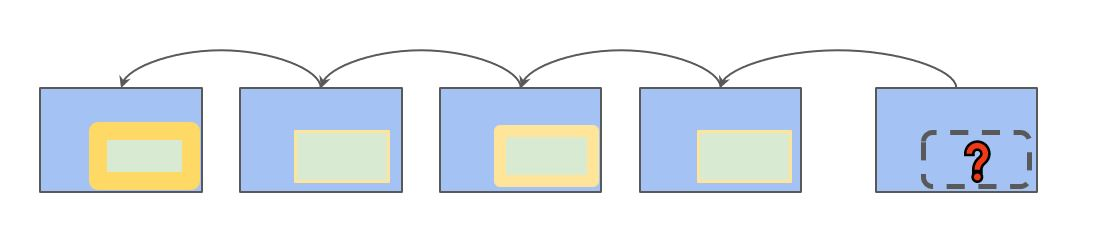
\includegraphics[width=0.8\linewidth]{Fig/22/F3}
		\caption{One possible way to implement PBS}
		\label{fig:L22_f3}
	\end{figure}
\end{center}
\subsection{How it works?}
The process is as follows:
\begin{itemize}
	\item The proposer broadcasts their query to the builder network, which is a network of nodes that want to buy blockspace for their transactions. The query contains information such as the available blockspace, the minimum bid, and the deadline for bidding.
	\item The builders respond to the query with their bids, which contain information such as the amount of blockspace they want, the price they are willing to pay, and the transactions they want to include.
	\item The proposer collects all the bids from the builder network and selects the highest bid that meets their criteria. The proposer then includes the transactions from the highest bidder in their own block and submits it to the block producer network.
	\item The block producer network validates and finalizes the block proposed by the proposer, without knowing or caring about the MEV involved in the transactions.
\end{itemize}
\subsection{Benefit On Decentralization}
PBS can promote decentralization in three ways:\\
\begin{enumerate}
	\item \textbf{Ethereum has a decentralized validator set:} This means that anyone who has enough stake, can become a validator and participate in the consensus process. PBS can encourage stakers of all sizes to join the network, as they do not have to compete for MEV opportunities or worry about re-org attacks. PBS can also prevent validator centralization, as users do not have to delegate their stake to validators who have more MEV resources or power.
	\item \textbf{Anyone can become a proposer} This means that anyone who can submit valid transactions can become a proposer and sell their blocks to builders who want to buy them. PBS can create a market for blockspace, where proposers can compete for MEV opportunities without affecting the block producers’ incentives or behavior. PBS can also increase the diversity and innovation of the network, as proposers can use different strategies and optimizations to order transactions.
	\item \textbf{The threat of re-org attacks reduces:} This means that validators have no incentive to fork the chain or withhold their blocks, since they do not benefit from MEV. PBS can reduce the risk of re-org attacks, as validators only care about validating and finalizing the blocks proposed by proposers. PBS can also improve the trust and reliability of the network, as users can have more confidence in the finality and validity of their transactions.
\end{enumerate}
\subsection{Issue: MEV stealing}
MEV stealing is when a validator takes the payload of a block proposed by a proposer and removes the builder who created it, and collects all the MEV for themselves. This can happen because validators have the power to decide which blocks to include or exclude from the chain, and they can also modify or reorder the transactions in the blocks. MEV stealing can harm the builders who invested their resources and time to assemble the payloads, and also reduce the efficiency and fairness of the market for blockspace.
Based on Figure \ref{fig:L22_f4}, MEV stealing can occur in three steps:
\begin{enumerate}
	\item Builders will take a “tip” to compensate them for their work of assembling the payloads: This means that builders will charge a fee for their service of creating blocks with optimal transaction ordering and MEV extraction. The fee can be paid by the proposers who buy their blocks, or by the users who submit their transactions to the builders.
	\item Validators can take payload, remove builder and collect all MEV: This means that validators can take advantage of the builders’ work and steal their blocks without paying them. Validators can do this by removing the builder’s address or signature from the block header, or by replacing the builder’s transactions with their own. Validators can then collect all the MEV from the transactions in the block, without sharing it with anyone else.
	\item Validators can propose their own blocks with stolen payloads: This means that validators can submit their own blocks with stolen payloads to the block producer network, and try to get them validated and finalized. Validators can do this by using their stake or resources to influence or bribe other validators, or by exploiting network or protocol vulnerabilities.
\end{enumerate}
\begin{center}
	\begin{figure}
		\centering
		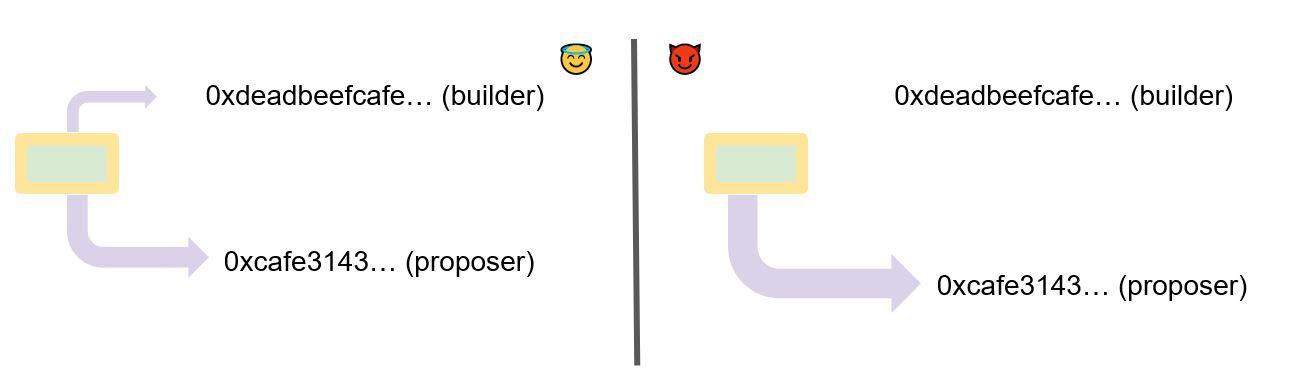
\includegraphics[width=0.8\linewidth]{Fig/22/F4}
		\caption{The diagram illustrates how MEV stealing can undermine the benefits of PBS, as it creates an incentive for validators to cheat and exploit the builders and proposers. MEV stealing can also affect the security and stability of the network, as it can cause forks, re-orgs, or censorship.}
		\label{fig:L22_f4}
	\end{figure}
\end{center}
\section{How to stop MEV stealing?}
We provide two possible solutions to stop MEV stealing, each with its own pros and cons:
\begin{enumerate}
	\item \textbf{Option 1:} Only allow trusted validators to access the network: This means that only validators who have a certain reputation or stake can propose or validate blocks, and they are expected to follow the honest protocol and respect the builders’ work. This option can prevent MEV stealing by creating a social contract or a legal agreement among the validators, and by imposing penalties or sanctions for any violations. However, this option also has some drawbacks, such as:
	\begin{itemize}
		\item It may be difficult to define and measure trust or reputation among validators, and to enforce or verify their compliance with the protocol or the agreement.
		\item Harms decentralization as only a subset of stakers can access profitable opportunities: It may reduce the diversity and participation of the network, as only a few validators can access the profitable MEV opportunities, creating an oligopoly or a monopoly.
		\item Some MEV opportunities can be larger than the ‘reputation’ built up so far: It may be possible that some validators are tempted to break their trust or reputation for a large MEV opportunity, especially if they think they can get away with it or if they plan to exit the network.
	\end{itemize}
	\item \textbf{Option 2:} Use a commit-and-reveal scheme: This means that validators have to commit their blocks before revealing their contents, and they cannot change or modify them after they are committed. This option can prevent MEV stealing by creating a cryptographic proof or a verifiable record of the blocks proposed by validators, and by making it impossible or costly for them to alter or replace them. However, this option also has some challenges, such as:
	\begin{itemize}
		\item It may require some technical modifications or innovations to implement such a scheme on the blockchain, such as using zero-knowledge proofs, secret sharing, or time-lock encryption.
		\item It may introduce some trade-offs between security, efficiency, and scalability, such as increasing the complexity, latency, or overhead of the protocol.
	\end{itemize}
\end{enumerate}

\section{Two-slot in-protocol PBS}
A two-slot in-protocol PBS is a scheme that uses two consecutive slots to allocate blockspace among proposers and builders, using a commit-and-reveal mechanism. A commit-and-reveal mechanism is a way of ensuring that validators cannot change or modify their blocks after they are committed, and they cannot see or copy other validators’ blocks before they are revealed, see Figure \ref{fig:L22_f5}. A two-slot in-protocol PBS works as follows:
\begin{enumerate}
	\item \textbf{Bidding phase:} In this phase, builders send bids to proposers, indicating how much they are willing to pay for blockspace and what transactions they want to include. The bids are encrypted and signed by the builders’ private keys. The proposers collect all the bids from the builders and select the highest bid that meets their criteria.
	\item \textbf{Bid selection (Slot 1):} In this slot, the proposer who selected the highest bid makes a beacon block, which is a block that contains only the hash of the bid and some other information, such as the proposer’s address and signature. The proposer commits their beacon block to the network, without revealing its contents. The beacon block serves as a proof that the proposer has selected a bid and cannot change it later.
	\item \textbf{Delivery (Slot 2):} In this slot, the builder who made the highest bid releases their block containing payload, which is a block that contains all the transactions from their bid and some other information, such as the builder’s address and signature. The builder reveals their block to the network, along with their bid and their private key. The builder’s block serves as a proof that the builder has paid for their blockspace and cannot be replaced by another builder.
\end{enumerate}
\begin{center}
	\begin{figure}
		\centering
		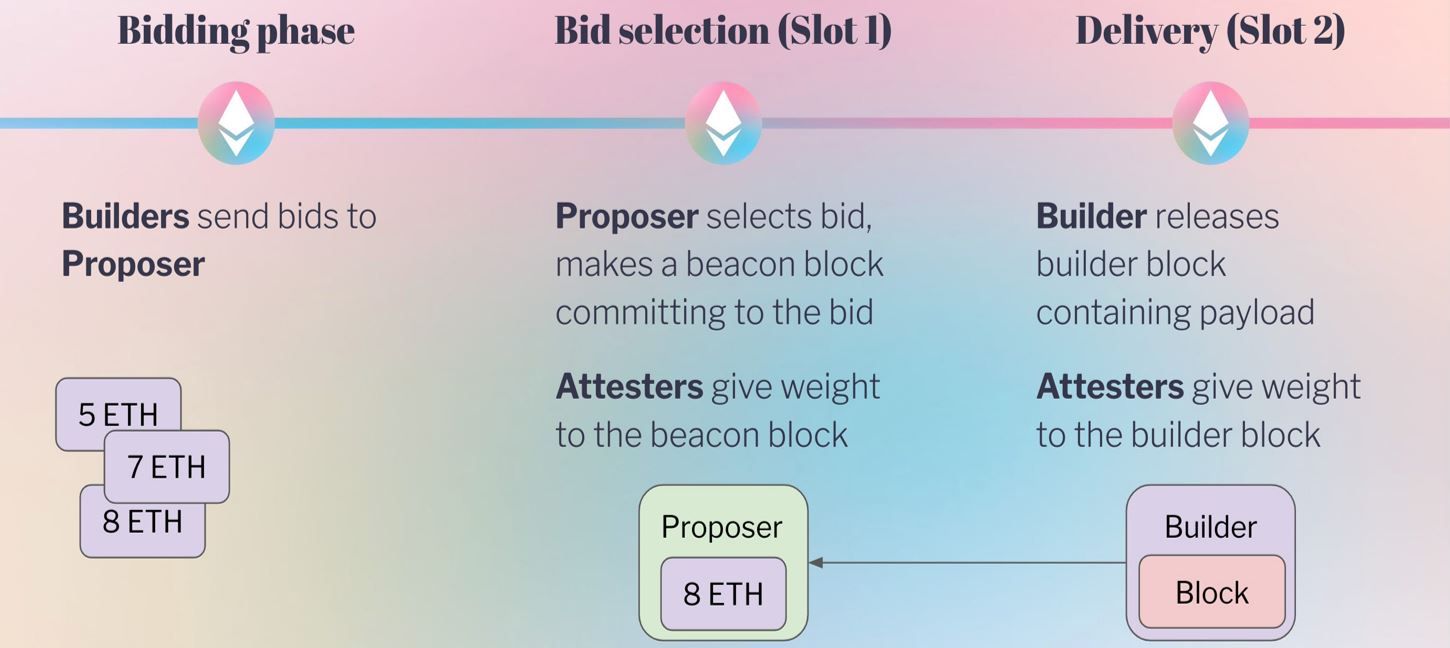
\includegraphics[width=1\linewidth]{Fig/22/F5}
		\caption{A two-slot in-protocol PBS can prevent MEV stealing by creating a cryptographic proof or a verifiable record of the blocks proposed by proposers and built by builders, and by making it impossible or costly for validators to alter or replace them.}
		\label{fig:L22_f5}
	\end{figure}
\end{center}
\subsection{Security Guarantees}
A two-slot in-protocol PBS can provide security guarantees to both builders and proposers, as follows:
\begin{itemize}
	\item \textbf{To the builder:} The document states that a commitment was entered into by the proposer, and that this commitment may only be revoked by a consensus failure. This means that once the proposer commits their beacon block to the network, they cannot change or modify it without breaking the protocol or causing a fork. This guarantees that the builder’s bid will not be stolen or replaced by another bid, unless there is a major disruption or attack on the network.
	\item \textbf{To the proposer:} The document states that the builder’s promise to honor the release no matter what the builder does, e.g., eventually fail to release the block contents or release an invalid block, in the latter case, the block is simply discarded, forcing the block builder to lose all transaction fees and MEV revenue. This means that once the builder reveals their block containing payload to the network, they cannot change or modify it without losing their payment or their reputation. This guarantees that the proposer will receive their payment for their blockspace allocation, unless there is a technical error or fraud on the builder’s part.
\end{itemize}
But there are some issues with the security guarantees in In-protocol PBS, as mentioned below:
\begin{enumerate}
	\item The fork choice rule would need to be updated: It may be necessary to update the fork choice rule, which is the rule that determines which chain is considered valid or canonical, to account for PBS. For example, one could use a longest-chain rule, where the chain with the most blocks is preferred, or a highest-bid rule, where the chain with the highest bid is preferred.
	\item The builder needs to be able to propose blocks: It may be challenging or impractical for builders to propose blocks to the network, as they may not have enough stake, resources, or connections to do so.
\end{enumerate}
\section{MEV-Boost}
MEV-Boost is a scheme that implements PBS outside of the consensus protocol, using a market mechanism and a probabilistic broadcast system. MEV-Boost can provide a working implementation of PBS, albeit with higher trust assumptions. MEV-Boost works in three steps:
\begin{itemize}
	\item \textbf{Builders and proposers do not necessarily trust each other:} This means that builders and proposers may have conflicting or competing interests or incentives, and they may not be willing to cooperate or share information with each other. For example, builders may want to maximize their MEV revenue, while proposers may want to minimize their blockspace cost.
	\item \textbf{Relays ensure:} This means that the relay can guarantee that the builders will not cheat or defraud the proposers by providing invalid or empty blocks. The relay can do this by requiring the builders to deposit some collateral or stake before submitting their bids, and by penalizing them if they fail to deliver their blocks or if their blocks are rejected by the network. The relay can also reward the builders if their blocks are accepted by the network.
\end{itemize}
\subsection{Architecture}
There are different components of the MEV-Boost architecture and how they interact with each other, see Figure \ref{fig:L22_f6}, \ref{fig:L22_f7}. The components are:
\begin{itemize}
	\item \textbf{Block builders:} These are the nodes that create blocks with optimal transaction ordering and MEV extraction. They can be anyone who can submit valid transactions, such as users, bots, or relays. The diagram shows three block builders, A, B, and C, who send their bids to the relay. The bids contain information such as the amount of blockspace they want, the price they are willing to pay, and the transactions they want to include.
	\item \textbf{Relay:} This is an external service or platform, such as Flashbots or MEV-Boost itself, that facilitates the communication and coordination between builders and proposers. The relay acts as a trusted intermediary that can collect bids from builders, select proposals from proposers, and match them together. The relay can also verify the validity and profitability of the bids and proposals, and ensure that they are executed on the network. The diagram shows the relay receiving bids from block builders and sending them to MEV-Boost.
	\item \textbf{MEV-Boost:} This is a software module that runs on top of the consensus protocol, such as Ethereum 2.0. It acts as a probabilistic broadcast system that can select and broadcast blocks to validators. It can also provide incentives or rewards for validators to include blocks proposed by proposers or built by builders. The diagram shows MEV-Boost receiving bids from the relay and selecting the most profitable block and the worst profitable block. The most profitable block is the one that has the highest bid or MEV revenue, while the worst profitable block is the one that has the lowest bid or MEV revenue.
	\item \textbf{Validator:} This is a node that validates and finalizes blocks on the blockchain. It can be anyone who has enough stake to participate in the consensus process. The diagram shows a validator receiving blocks from MEV-Boost and including them in their own proposals.
\end{itemize}
\begin{center}
	\begin{figure}
		\centering
		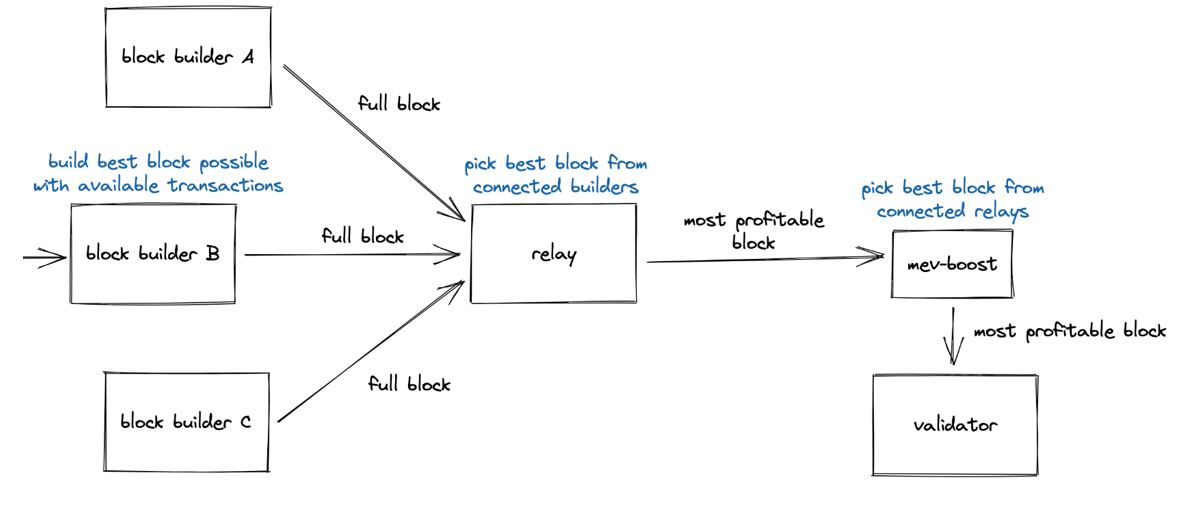
\includegraphics[width=1\linewidth]{Fig/22/F6}
		\caption{The diagram illustrates how MEV-Boost can implement PBS outside of the consensus protocol, by using a market mechanism and a probabilistic broadcast system to allocate blockspace among builders and proposers.}
		\label{fig:L22_f6}
	\end{figure}
\end{center}
\begin{center}
	\begin{figure}
		\centering
		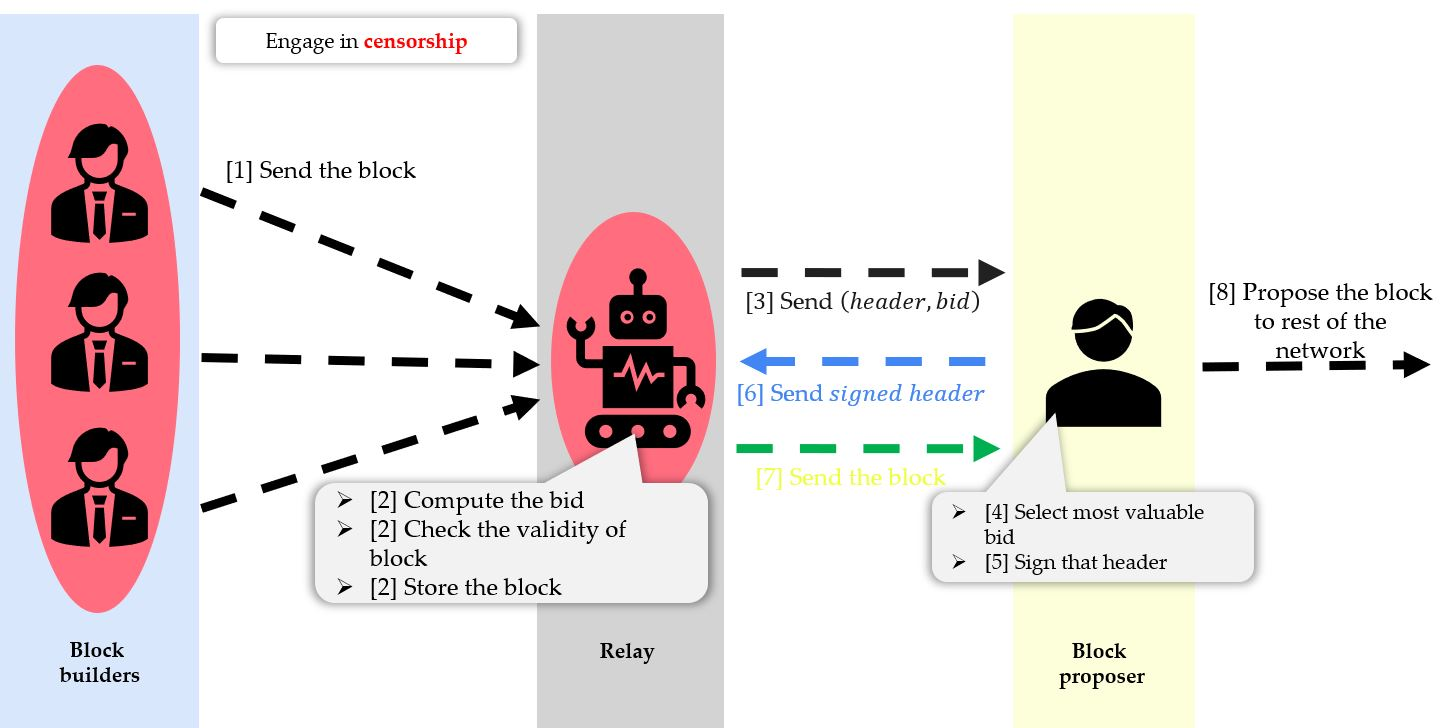
\includegraphics[width=1\linewidth]{Fig/22/F7}
		\caption{MEV-Boost process and architecture.}
		\label{fig:L22_f7}
	\end{figure}
\end{center}
\section{Censorship}
As mentioned above, transaction censorship is when a validator or a miner decides to exclude or delay certain transactions from being included in a block, based on their own preferences or incentives. Transaction censorship can harm the users who submitted the transactions, and also reduce the efficiency and fairness of the network.
Censorship is implemented in two ways: \textbf{inclusion lists} and \textbf{proposer suffixes}
\subsection{Inclusion Lists}
Inclusion lists are a way of allowing users to specify which transactions they demand must be included in a block, and preventing validators or miners from censoring them, see Figure \ref{fig:L22_f8}. Inclusion lists work as follows:\\
\begin{itemize}
	\item A proposer provides an inclusion list, a list of transactions they demand must be included in the block: This means that a user who wants to submit a transaction can also provide an inclusion list, which is a list of other transactions that they want to see in the same block as their transaction. The inclusion list can be based on the user’s own interests or preferences, such as supporting certain projects, causes, or communities. The inclusion list can also be based on the user’s own security or privacy, such as avoiding front-running, back-running, or sandwich attacks.
	\item Unless the builder can fill a block completely with other transactions: This means that a validator or a miner who wants to create a block can either respect the inclusion list provided by the proposer, or ignore it and fill the block with other transactions. However, if they choose to ignore the inclusion list, they have to fill the entire block with other transactions, leaving no space for any transaction from the inclusion list. This creates a trade-off for the validator or miner, as they have to weigh the benefits and costs of including or excluding the inclusion list.
	\item The proposer can verify that their inclusion list was respected by checking the block: This means that once the block is created and broadcasted to the network, the proposer can check if their inclusion list was respected by the validator or miner. If their inclusion list was respected, they can be satisfied that their transaction and their preferred transactions were included in the block. If their inclusion list was ignored, they can be disappointed that their transaction and their preferred transactions were excluded from the block.
\end{itemize}
\begin{center}
	\begin{figure}
		\centering
		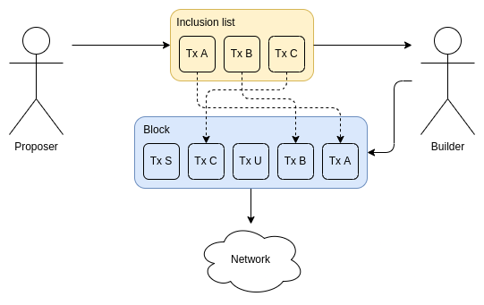
\includegraphics[width=0.7\linewidth]{Fig/22/F8}
		\caption{The diagram below is an explanation of censorship resistance via inclusion lists, which is a possible solution to the problem of transaction censorship on the blockchain.}
		\label{fig:L22_f8}
	\end{figure}
\end{center}
\subsection{Proposer Suffixes}
Proposer suffixes are a way of allowing users to add some transactions to the end of a block, after the block has been created by a builder, see Figure \ref{fig:L22_f9}. Proposer suffixes work as follows:\\
\begin{itemize}
	\item An alternative approach is to allow the proposer to create a suffix for the block: This means that a user who wants to submit a transaction can also create a suffix, which is a list of transactions that they want to add to the end of the block. The suffix can be based on the user’s own interests or preferences, such as supporting certain projects, causes, or communities. The suffix can also be based on the user’s own security or privacy, such as avoiding front-running, back-running, or sandwich attacks.
	\item The proposer sends the block and the suffix to the network: This means that once the user has created their suffix, they can send it along with the block that they have received from the builder. The block and the suffix are broadcasted to the network, and other validators or miners can see them and include them in their own proposals.
	\item The proposer can verify that their suffix was respected by checking the block: This means that once the block and the suffix are included in the chain, the user can check if their suffix was respected by the validator or miner. If their suffix was respected, they can be satisfied that their transaction and their preferred transactions were included in the block. If their suffix was ignored, they can be disappointed that their transaction and their preferred transactions were excluded from the block.
\end{itemize}
\begin{center}
	\begin{figure}
		\centering
		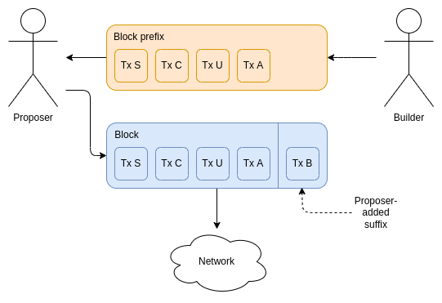
\includegraphics[width=0.7\linewidth]{Fig/22/F9}
		\caption{The diagram illustrates how proposer suffixes can provide censorship resistance to users, as they can express their preferences and demands for blockspace allocation, and prevent validators or miners from censoring them.}
		\label{fig:L22_f9}
	\end{figure}
\end{center}
\textbf{Pre-commitment} is a scheme that prevents MEV stealing by proposers, by requiring them to commit to a set of transactions that they want to include in the suffix, before they receive the block from the builder, see Figure \ref{fig:L22_f10}. Pre-commitment works as follows:
\begin{itemize}
	\item The proposer pre-commits to a Merkle tree or KZG commitment or other accumulator of the set of transactions they want to include: This means that a user who wants to create a suffix for a block has to generate a cryptographic proof or a verifiable record of the set of transactions that they want to include in the suffix. The proof can be based on different techniques, such as Merkle trees, KZG commitments, or other accumulators. The proof can be verified by anyone who knows the set of transactions and the proof itself.
	\item The proposer sends the pre-commitment to the network: This means that once the user has generated their proof, they have to broadcast it to the network, and make it visible and accessible to everyone. The pre-commitment serves as a proof that the user has selected a set of transactions and cannot change it later.
	\item The proposer receives the block from the builder and adds it to the suffix tree: This means that once the user receives the block from the builder, they have to add it to their suffix tree, which is a data structure that stores the blocks and their suffixes. The user can only add the block if it matches their pre-commitment, otherwise they have to discard it.
	\item The proposer sends the block and the suffix to the network: This means that once the user has added the block to their suffix tree, they have to send it along with their suffix to the network. The block and the suffix are broadcasted to the network, and other validators or miners can see them and include them in their own proposals.
\end{itemize}
\begin{center}
	\begin{figure}
		\centering
		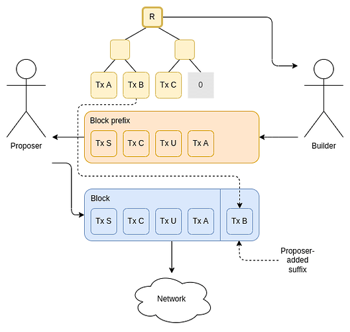
\includegraphics[width=0.6\linewidth]{Fig/22/F10}
		\caption{The diagram illustrates how pre-commitment can prevent MEV stealing by proposers, by creating a cryptographic proof or a verifiable record of the set of transactions that they want to include in the suffix, and by making it impossible or costly for them to alter or replace them.}
		\label{fig:L22_f10}
	\end{figure}
\end{center}